% GNUPLOT: LaTeX picture with Postscript

\definecolor{BL}{rgb}{0, 0.4470, 0.7410}
\definecolor{OR}{rgb}{0.6500, 0.3250, 0.1980}
\definecolor{GR}{rgb}{0.4660, 0.7740, 0.2880}
\definecolor{PU}{rgb}{0.4940, 0.1840, 0.5560}

\begingroup
  \makeatletter
  \providecommand\color[2][]{%
    \GenericError{(gnuplot) \space\space\space\@spaces}{%
      Package color not loaded in conjunction with
      terminal option `colourtext'%
    }{See the gnuplot documentation for explanation.%
    }{Either use 'blacktext' in gnuplot or load the package
      color.sty in LaTeX.}%
    \renewcommand\color[2][]{}%
  }%
  \providecommand\includegraphics[2][]{%
    \GenericError{(gnuplot) \space\space\space\@spaces}{%
      Package graphicx or graphics not loaded%
    }{See the gnuplot documentation for explanation.%
    }{The gnuplot epslatex terminal needs graphicx.sty or graphics.sty.}%
    \renewcommand\includegraphics[2][]{}%
  }%
  \providecommand\rotatebox[2]{#2}%
  \@ifundefined{ifGPcolor}{%
    \newif\ifGPcolor
    \GPcolorfalse
  }{}%
  \@ifundefined{ifGPblacktext}{%
    \newif\ifGPblacktext
    \GPblacktexttrue
  }{}%
  % define a \g@addto@macro without @ in the name:
  \let\gplgaddtomacro\g@addto@macro
  % define empty templates for all commands taking text:
  \gdef\gplfronttext{}%
  \gdef\gplfronttext{}%
  \makeatother
  \ifGPblacktext
    % no textcolor at all
    \def\colorrgb#1{}%
    \def\colorgray#1{}%
  \else
    % gray or color?
    \ifGPcolor
      \def\colorrgb#1{\color[rgb]{#1}}%
      \def\colorgray#1{\color[gray]{#1}}%
      \expandafter\def\csname LTw\endcsname{\color{white}}%
      \expandafter\def\csname LTb\endcsname{\color{black}}%
      \expandafter\def\csname LTa\endcsname{\color{black}}%
      \expandafter\def\csname LT0\endcsname{\color[rgb]{1,0,0}}%
      \expandafter\def\csname LT1\endcsname{\color[rgb]{0,1,0}}%
      \expandafter\def\csname LT2\endcsname{\color[rgb]{0,0,1}}%
      \expandafter\def\csname LT3\endcsname{\color[rgb]{1,0,1}}%
      \expandafter\def\csname LT4\endcsname{\color[rgb]{0,1,1}}%
      \expandafter\def\csname LT5\endcsname{\color[rgb]{1,1,0}}%
      \expandafter\def\csname LT6\endcsname{\color[rgb]{0,0,0}}%
      \expandafter\def\csname LT7\endcsname{\color[rgb]{1,0.3,0}}%
      \expandafter\def\csname LT8\endcsname{\color[rgb]{0.5,0.5,0.5}}%
    \else
      % gray
      \def\colorrgb#1{\color{black}}%
      \def\colorgray#1{\color[gray]{#1}}%
      \expandafter\def\csname LTw\endcsname{\color{white}}%
      \expandafter\def\csname LTb\endcsname{\color{black}}%
      \expandafter\def\csname LTa\endcsname{\color{black}}%
      \expandafter\def\csname LT0\endcsname{\color{black}}%
      \expandafter\def\csname LT1\endcsname{\color{black}}%
      \expandafter\def\csname LT2\endcsname{\color{black}}%
      \expandafter\def\csname LT3\endcsname{\color{black}}%
      \expandafter\def\csname LT4\endcsname{\color{black}}%
      \expandafter\def\csname LT5\endcsname{\color{black}}%
      \expandafter\def\csname LT6\endcsname{\color{black}}%
      \expandafter\def\csname LT7\endcsname{\color{black}}%
      \expandafter\def\csname LT8\endcsname{\color{black}}%
    \fi
  \fi
    \setlength{\unitlength}{0.0500bp}%
    \ifx\gptboxheight\undefined%
      \newlength{\gptboxheight}%
      \newlength{\gptboxwidth}%
      \newsavebox{\gptboxtext}%
    \fi%
    \setlength{\fboxrule}{0.5pt}%
    \setlength{\fboxsep}{1pt}%
\begin{picture}(5000.00,5000.00)%
    \gplgaddtomacro\gplfronttext{%
    }%
    \gplgaddtomacro\gplfronttext{%
      \colorrgb{0.00,0.00,0.00}%
      \put(1175,4600){\makebox(0,0)[l]{\strut{}$\small \mathcal{S}_R$}}%
      \colorrgb{0.00,0.00,0.00}%
      \put(1175,4349){\makebox(0,0)[l]{\strut{}$\small \mathcal{S}_V^0(\hat{\theta}+0\frac{\gamma}{2^2})$}}%
      \colorrgb{0.00,0.45,0.74}%
      \put(1379,3945){\makebox(0,0)[l]{\color{BL}\strut{}\small $\texttt{PD}^{(2)}_0$$=0.96$}}%
    }%
    \gplgaddtomacro\gplfronttext{%
    }%
    \gplgaddtomacro\gplfronttext{%
      \colorrgb{0.00,0.00,0.00}%
      \put(3625,4600){\makebox(0,0)[l]{\strut{}\small $\mathcal{S}_R$}}%
      \colorrgb{0.00,0.00,0.00}%
      \put(3625,4349){\makebox(0,0)[l]{\strut{}\small $\mathcal{S}_V^1(\hat{\theta}+1\frac{\gamma}{2^2})$}}%
      \colorrgb{0.65,0.33,0.20}%
      \put(3829,3945){\makebox(0,0)[l]{\color{OR}\strut{}\small $\texttt{PD}^{(2)}_1$$=0.90$}}%
    }%
    \gplgaddtomacro\gplfronttext{%
    }%
    \gplgaddtomacro\gplfronttext{%
      \colorrgb{0.00,0.00,0.00}%
      \put(1175,2150){\makebox(0,0)[l]{\strut{}\small $\mathcal{S}_R$}}%
      \colorrgb{0.00,0.00,0.00}%
      \put(1175,1899){\makebox(0,0)[l]{\strut{}\small $\mathcal{S}_V^2(\hat{\theta}+2\frac{\gamma}{2^2})$}}%
      \colorrgb{0.47,0.77,0.29}%
      \put(1379,1495){\makebox(0,0)[l]{\color{GR}\small \strut{}$\texttt{PD}^{(2)}_2$$=0.92$}}%
    }%
    \gplgaddtomacro\gplfronttext{%
    }%
    \gplgaddtomacro\gplfronttext{%
      \colorrgb{0.00,0.00,0.00}%
      \put(3625,2150){\makebox(0,0)[l]{\strut{}\small $\mathcal{S}_R$}}%
      \colorrgb{0.00,0.00,0.00}%
      \put(3625,1899){\makebox(0,0)[l]{\strut{}\small $\mathcal{S}_V^3(\hat{\theta}+3\frac{\gamma}{2^2})$}}%
      \colorrgb{0.49,0.18,0.56}%
      \put(3829,1495){\makebox(0,0)[l]{\color{PU}\small \strut{}$\texttt{PD}^{(2)}_3$$=0.99$}}%
    }%
    \put(0,0){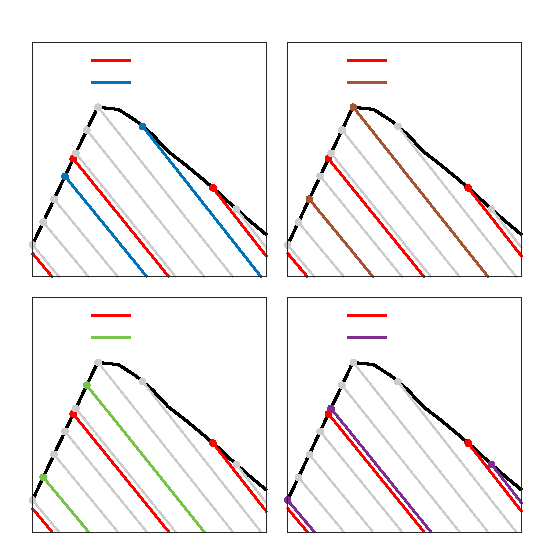
\includegraphics{./figures/parts/02/chapters/04/sections/02/correct_oversampling}}%
    \gplfronttext
  \end{picture}%
\endgroup
